\documentclass[a4paper,10pt,oneside,leqno]{scrartcl}
\usepackage[utf8]{inputenc}
\usepackage{listingsutf8}
\usepackage[pdftex]{graphicx}
%\usepackage[ngerman]{babel}
\usepackage{url}
\usepackage{hyperref}
\usepackage{amsfonts}
\usepackage{amssymb}
\usepackage{amsmath}
\usepackage{tikz}
\usepackage{listings}
\usepackage{pdfpages}
\usepackage{textcomp}
\usepackage{amsmath}
%\usepackage{lipsum}%%%%%%%%%%%%%%%%%%%%%%%%%%%%%%%%%%%%%%%%%%%%%%%%%%%%%%%%%%%%%%%%%%%%%%%%%%%%%%%%%%%%
\usepackage{mathtools}
\usepackage{amsfonts}
\usepackage{amssymb}
\usepackage{amsmath}
\usepackage{booktabs}
%usepackage[utf8x]{inputenc}
\usepackage[T1]{fontenc}
\usepackage{lmodern} %Latin modern = enhanced CM font
\usepackage{xspace} %Space enhancements
%\usepackage{algorithmic}%%%%%%%%%%%%%%%%%%%%%%%%%%%%%%%%%%%%%%%%%%%%%%%%%%%%%%%%%%%%%%%%%%%%%%%%%%%%%%%%%%
%\usepackage{algpseudocode}

\usepackage[paper=a4paper,includefoot,includehead,left=30mm,right=20mm,top=20mm,bottom=20mm]{geometry}
%opening
\title{Übungsblatt 5}
\author{Uli Köhler (10580373), Tobias Harrer (10575835)}
\begin{document}

\maketitle

\section*{Aufgabe 1}%T
siehe schriftlich (auf den letzten Seiten)

\section*{Aufgabe 2}%U
\subsection*{Teilaufgabe a)}
Per def. gilt: $d(A,B) = max\{a, b:x\in a, \wedge b \in B\}$

\begin{align}
 d(X,Y) &=& max\{d(x,y):x\in X \wedge y \in Y\}\\
 &=& max\{d(x,y):x\in A\cup B \wedge y \in Y\}\\
 &=& max(\{d(x,y):x\in A \wedge y \in Y\} \cup \{d(x,y):x\in B \wedge y \in Y\})\\
 &=& max(d(A,Y), d(B,Y))
\end{align}

\subsection*{Teilaufgabe B)}
$d(X,Y) = \frac{\Sigma_{x \in X}\Sigma_{y \in Y}d(x,y)}{|X|\times |Y|}
=\frac{\Sigma_{x \in A\cup B}\Sigma_{y \in Y}d(x,y)}{|A\cup B|\times |Y|}$\\
$=\frac{\Sigma_{x \in A}\Sigma_{y \in Y}d(x,y) + \Sigma_{x \in B}\Sigma_{y \in Y}d(x,y)}{(|A| + |B|)\times |Y|}$
(wobei gerade $|A| + |B| = |A \cup B|$ da $|A \cap B| = 0$)\\

\[
 =\frac{\frac{\Sigma_{x \in A}\Sigma_{y \in Y}d(x,y)}{|A|\times |Y|} |A|\times|Y| + \frac{\Sigma_{x B}\Sigma_{y \in Y}d(x,y)}{|B|\times |Y|} |B|\times|Y|}{(|A|+|B|)\times |Y|}
\]

Nach Kürzung ergibt sich

\[
 \frac{|A|d(A,Y) + |B|d(B,Y)}{|A| + |B|}
\]

q.e.d


\section*{Aufgabe 3}%U
Siehe schriftlich:

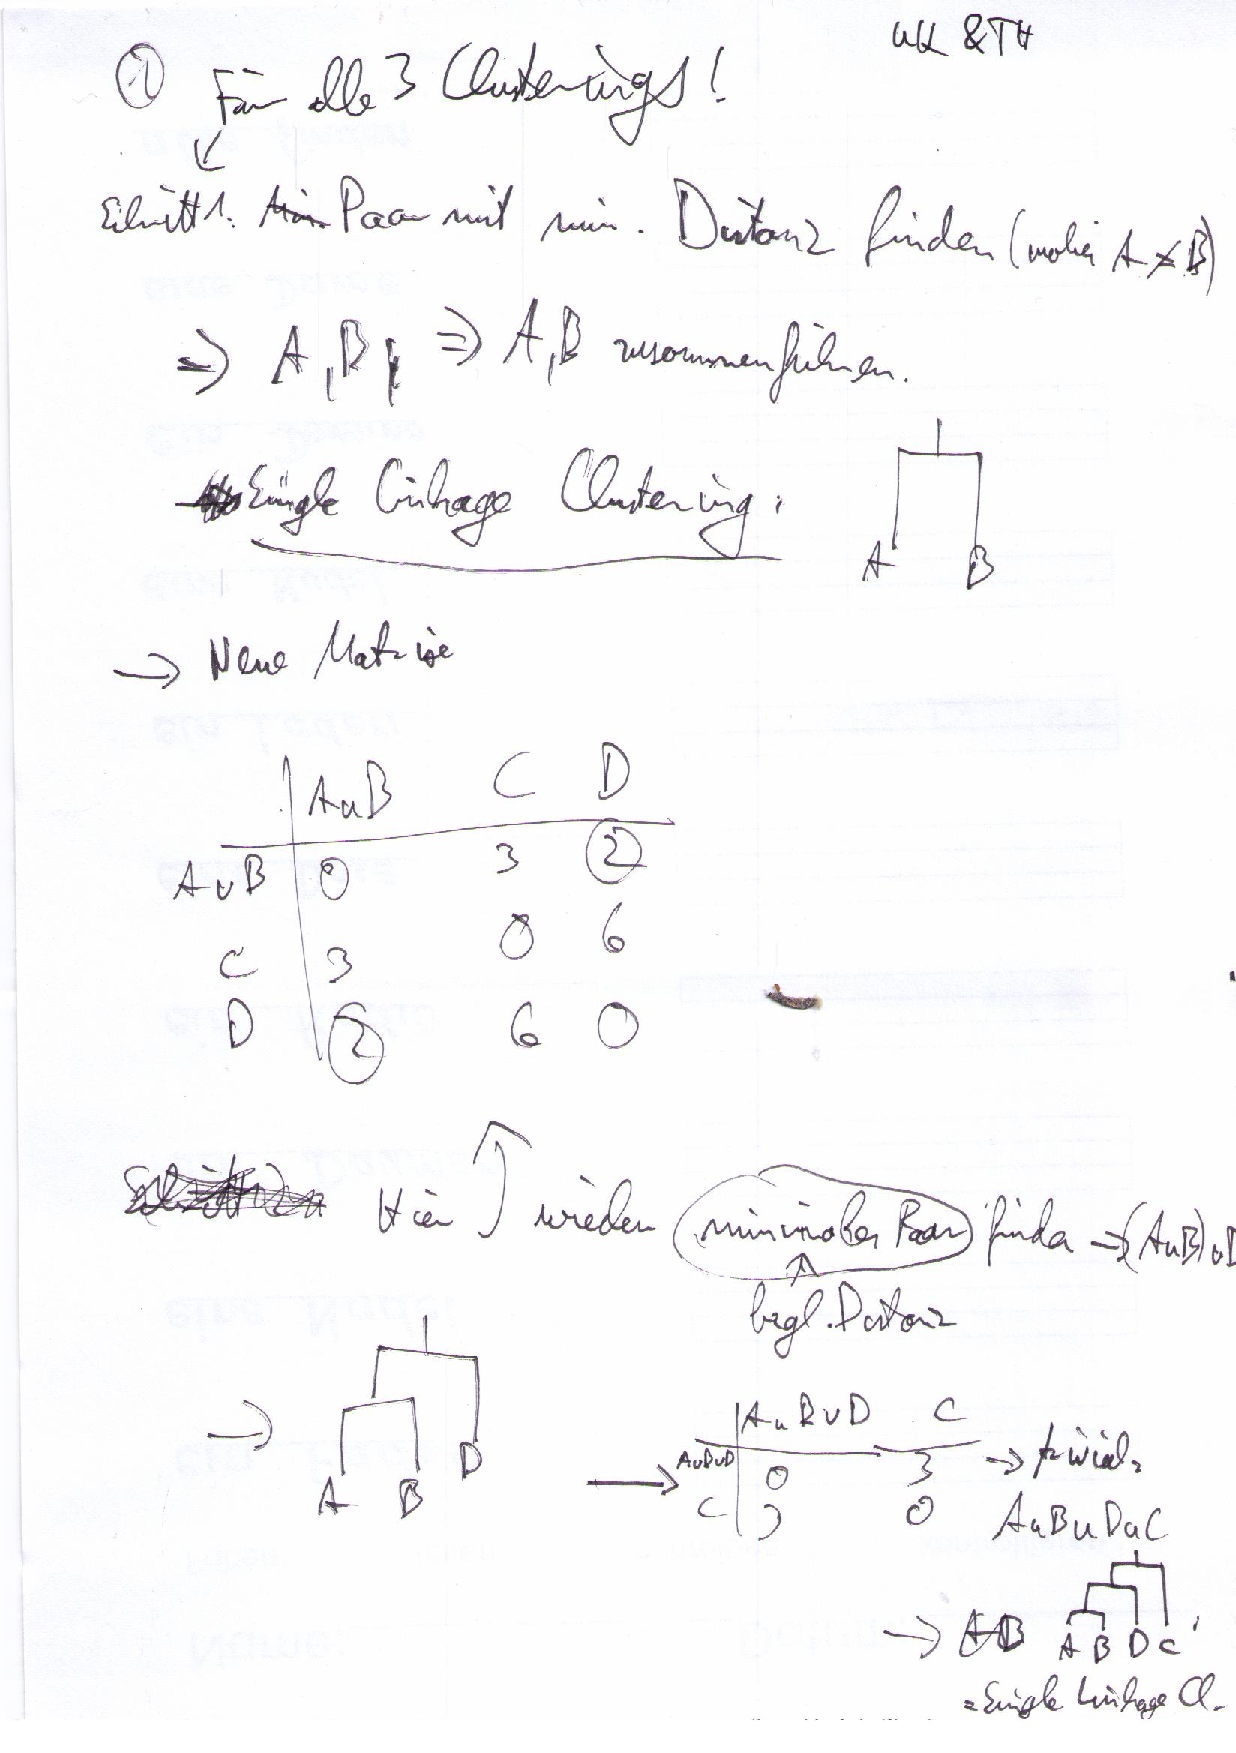
\includepdf[pages=-]{A3.pdf}

%\section*{Aufgabe 4}%T


\end{document}
















